% !TEX root = ../mechanics.tex
\chapter{不可压无粘流绕流有限翼展的机翼}
前面介绍了无限翼展的翼型气动特性,这一章主
要介绍有限翼展的机翼的气动特性。
\section{下洗和诱导阻力}
有限翼展的机翼是三维的,所以机翼的气动特性
和翼型的气动特性不同,如下图\ref{fig:span}。
\begin{figure}[!ht]
  \centering 
  % ! TEX root = ./aerodynamics/finite_wing.tex
\tikzset{every picture/.style={line width=0.75pt}} %set default line width to 0.75pt        

\begin{tikzpicture}[x=0.75pt,y=0.75pt,yscale=-1,xscale=1]
%uncomment if require: \path (0,379); %set diagram left start at 0, and has height of 379

%Straight Lines [id:da39727047577203534] 
\draw [line width=1.5]    (60,150) -- (60,230) ;
%Straight Lines [id:da11447013885536217] 
\draw [line width=1.5]    (520,150) -- (520,230) ;
%Straight Lines [id:da1723130381460103] 
\draw [line width=1.5]    (60,150) -- (290,120) ;
%Straight Lines [id:da8684705023837216] 
\draw [line width=1.5]    (290,260) -- (520,230) ;
%Straight Lines [id:da6095913924584648] 
\draw [line width=1.5]    (290,120) -- (520,150) ;
%Straight Lines [id:da8952813053936264] 
\draw [line width=1.5]    (60,230) -- (290,260) ;
%Straight Lines [id:da7569741842644373] 
\draw    (60,280) -- (60,320) ;
%Straight Lines [id:da053098603590512106] 
\draw    (520,280) -- (520,320) ;
%Straight Lines [id:da3779632700211717] 
\draw    (290,300) -- (62,300) ;
\draw [shift={(60,300)}, rotate = 360] [color={rgb, 255:red, 0; green, 0; blue, 0 }  ][line width=0.75]    (10.93,-3.29) .. controls (6.95,-1.4) and (3.31,-0.3) .. (0,0) .. controls (3.31,0.3) and (6.95,1.4) .. (10.93,3.29)   ;
%Straight Lines [id:da20615235094281092] 
\draw    (290,300) -- (518,300) ;
\draw [shift={(520,300)}, rotate = 180] [color={rgb, 255:red, 0; green, 0; blue, 0 }  ][line width=0.75]    (10.93,-3.29) .. controls (6.95,-1.4) and (3.31,-0.3) .. (0,0) .. controls (3.31,0.3) and (6.95,1.4) .. (10.93,3.29)   ;
%Straight Lines [id:da791640112777152] 
\draw    (290,190) -- (290,258) ;
\draw [shift={(290,260)}, rotate = 270] [color={rgb, 255:red, 0; green, 0; blue, 0 }  ][line width=0.75]    (10.93,-3.29) .. controls (6.95,-1.4) and (3.31,-0.3) .. (0,0) .. controls (3.31,0.3) and (6.95,1.4) .. (10.93,3.29)   ;
%Straight Lines [id:da325406846820093] 
\draw    (290,190) -- (290,122) ;
\draw [shift={(290,120)}, rotate = 90] [color={rgb, 255:red, 0; green, 0; blue, 0 }  ][line width=0.75]    (10.93,-3.29) .. controls (6.95,-1.4) and (3.31,-0.3) .. (0,0) .. controls (3.31,0.3) and (6.95,1.4) .. (10.93,3.29)   ;
%Straight Lines [id:da8596149068704069] 
\draw    (210,130) -- (210,250) ;
%Straight Lines [id:da41281193810683314] 
\draw    (540,150) -- (580,150) ;
%Straight Lines [id:da047103836611672945] 
\draw    (540,230) -- (580,230) ;
%Straight Lines [id:da16724290585118085] 
\draw    (560,190) -- (560,228) ;
\draw [shift={(560,230)}, rotate = 270] [color={rgb, 255:red, 0; green, 0; blue, 0 }  ][line width=0.75]    (10.93,-3.29) .. controls (6.95,-1.4) and (3.31,-0.3) .. (0,0) .. controls (3.31,0.3) and (6.95,1.4) .. (10.93,3.29)   ;
%Straight Lines [id:da35748881145221234] 
\draw    (560,190) -- (560,152) ;
\draw [shift={(560,150)}, rotate = 90] [color={rgb, 255:red, 0; green, 0; blue, 0 }  ][line width=0.75]    (10.93,-3.29) .. controls (6.95,-1.4) and (3.31,-0.3) .. (0,0) .. controls (3.31,0.3) and (6.95,1.4) .. (10.93,3.29)   ;
%Straight Lines [id:da7041026114003535] 
\draw    (290,30) -- (290,98) ;
\draw [shift={(290,100)}, rotate = 270] [color={rgb, 255:red, 0; green, 0; blue, 0 }  ][line width=0.75]    (10.93,-3.29) .. controls (6.95,-1.4) and (3.31,-0.3) .. (0,0) .. controls (3.31,0.3) and (6.95,1.4) .. (10.93,3.29)   ;
%Curve Lines [id:da3986433821781994] 
\draw    (130,40) .. controls (134.84,120.2) and (130.9,216.64) .. (189.12,269.21) ;
\draw [shift={(190,270)}, rotate = 221.54] [color={rgb, 255:red, 0; green, 0; blue, 0 }  ][line width=0.75]    (10.93,-3.29) .. controls (6.95,-1.4) and (3.31,-0.3) .. (0,0) .. controls (3.31,0.3) and (6.95,1.4) .. (10.93,3.29)   ;
%Curve Lines [id:da7469912525973164] 
\draw  [dash pattern={on 4.5pt off 4.5pt}]  (160,40) .. controls (163.83,129.7) and (157,242.33) .. (111.39,269.21) ;
\draw [shift={(110,270)}, rotate = 331.55] [color={rgb, 255:red, 0; green, 0; blue, 0 }  ][line width=0.75]    (10.93,-3.29) .. controls (6.95,-1.4) and (3.31,-0.3) .. (0,0) .. controls (3.31,0.3) and (6.95,1.4) .. (10.93,3.29)   ;

% Text Node
\draw (409,169) node [anchor=north west][inner sep=0.75pt]   [align=left] {机翼面积$\displaystyle S$};
% Text Node
\draw (298,187) node [anchor=north west][inner sep=0.75pt]   [align=left] {$\displaystyle C_{r}$};
% Text Node
\draw (529,169) node [anchor=north west][inner sep=0.75pt]   [align=left] {翼\\尖};
% Text Node
\draw (259,167) node [anchor=north west][inner sep=0.75pt]   [align=left] {翼\\根};
% Text Node
\draw (179,149) node [anchor=north west][inner sep=0.75pt]   [align=left] {平\\均\\弦\\长};
% Text Node
\draw (255,268) node [anchor=north west][inner sep=0.75pt]   [align=left] {翼展};
% Text Node
\draw (269,309) node [anchor=north west][inner sep=0.75pt]    {$b$};
% Text Node
\draw (569,177) node [anchor=north west][inner sep=0.75pt]    {$C_{t}$};
% Text Node
\draw (299,49) node [anchor=north west][inner sep=0.75pt]   [align=left] {自由来流$\displaystyle V_{\infty }$};


\end{tikzpicture}

  \caption{机翼}
  \label{fig:span}
\end{figure}
在上图中,实线代表机翼上方气流的流动情况;
虚线代表机翼下方气流的流动情况。

下面先介绍几个概念。{\bfseries 翼展(span)}$b$
是机翼两个翼尖之间的距离。{\bfseries 平均弦
长}$c$即机翼的平均气动弦长。对于矩形机翼来说,
机翼的弦长都相等,所以平均气动弦长也等于翼型
的弦长。{\bfseries 后掠角}$\chi$机翼前缘和机身纵轴
的夹角。{\bfseries 根稍比}$\eta$机翼根部的弦长和翼
尖的弦长的比值,$\eta=\frac{c_r}{c_t}$。{\bfseries 
展弦比}$\lambda$,机翼翼展和平均气动弦长的比值。
机翼的面积$S=bc$,即平均气动弦长和翼展乘积。所以
展弦比也等于$\lambda=\frac{b^2}{S}$。

暂时,可以将机翼产生升力的原因归结于机翼下表面的
压强比上表面的大,所以机翼受到一个向上的压强力,
即升力。在翼尖处,由于机翼下表面的压强大于上表面,
所以气流就会这压强的推动下,向上流动,这就是为什么
下表面的气流会向翼尖处流动,而上表面的气流会向翼根
处流动。
\begin{note}
升力产生的原因不全是压强差的问题,还有牛顿第三定律的缘故。
关于压强差产生的原因,不能完全用伯努利方程解释,但确实机翼
上表面的流速大于下表面的流速,参考上一章讨论翼型的升力。
\end{note}
翼尖处气流向上流动,形成了一个涡,这个涡叫做
{\bfseries 翼尖涡(wing-tip vortice)},也叫
{\bfseries 尾涡(trailing vortex)}。
\begin{note}
对于一些大飞机,比如Boeing 747,它们产生的翼尖涡非常
强大,会使得跟得太近的小飞机失控,从而导致事故。
\end{note}
这些翼尖涡会诱导一个小的向下的速度,也就是下洗,用
符号$w$表示。相应地,下洗的速度$w$和自由来流的速度$V_\infty$
的合速度就是流过机翼翼型的实际速度。

自由来流和翼型弦线的夹角叫做攻角,这里我们记为{\bfseries 几何攻角
(geometric angle of attack)}
$\alpha$,如图\ref{fig:effective_attack}
\begin{figure}[!ht]
  \centering
  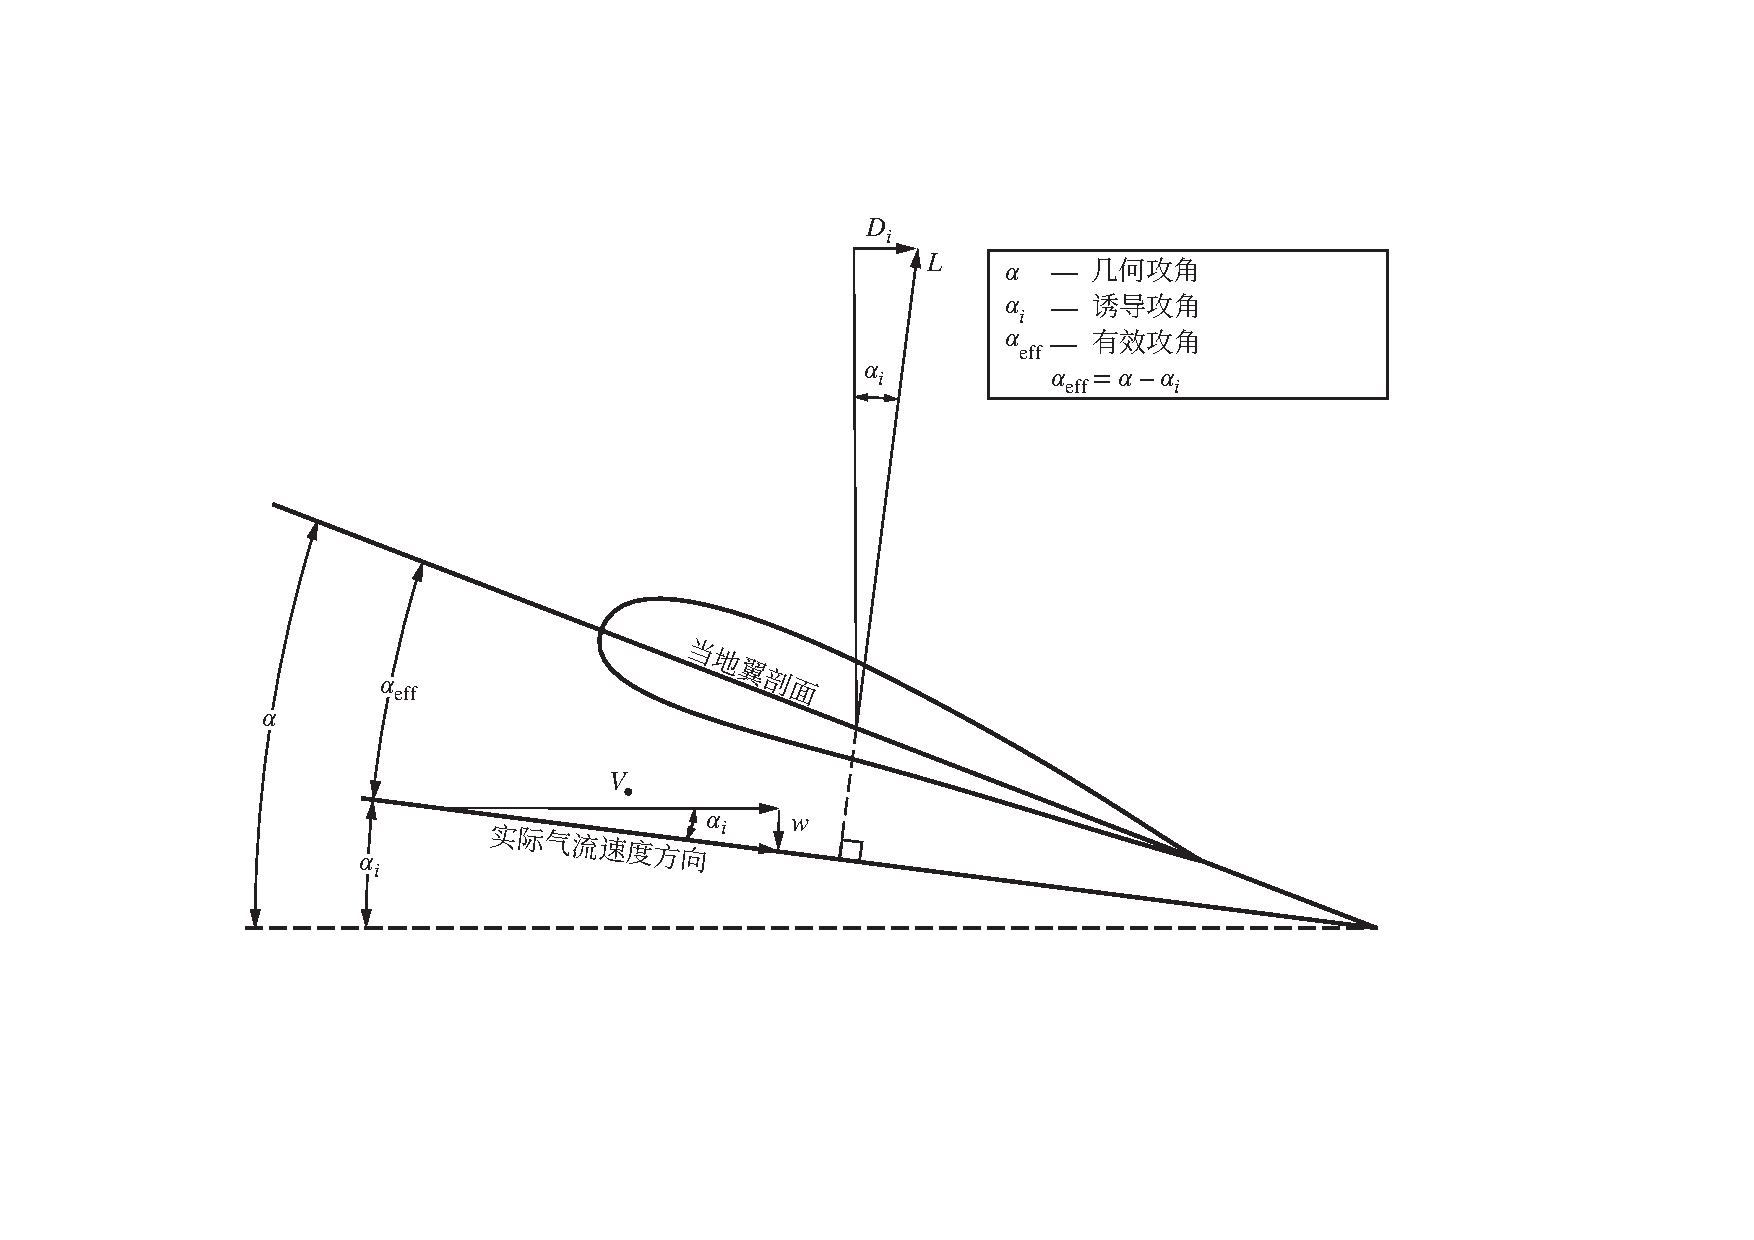
\includegraphics[height=10cm]{./aerodynamics/effective_attack.pdf}
  \caption{下洗对有限翼展机翼当地翼型截面的影响}
  \label{fig:effective_attack}
\end{figure}
当地气流的方向相对于自由来流的方向向下倾斜了$\alpha_i$角度,这个角度
叫做{\bfseries 诱导攻角(induced angle of attack)}。下洗流的存在,
使得当地气流方向向下倾斜,同时对当地翼有剖面主要有两个
影响,如下:
\begin{enumerate}
  \item 实际的迎角是当地气流的方向和当地翼型弦线的夹角,这个夹角
    叫做{\bfseries 有效迎角(effective angle of attack)},记作
    $\alpha_{eff}$。因此,即使机翼有着几何攻角$\alpha$,当地翼型的
    迎角实际上更下一些,即有效迎角。
    \[
      \alpha_{eff}=\alpha-\alpha_i
    \]
  \item 当地的升力向量垂直于当地气流方向,因此相较于原来的升力向量
    (竖直方向)落后了角度$\alpha_i$。结果是在自由来流的方向会有
    一个当地升力向量的分量。也就是说,这个阻力是因为下洗的原因产生
    的。这个阻力就被叫做{\bfseries 诱导阻力(induced drag)},记作
    $D_i$。
\end{enumerate}

升力向后倾斜是诱导阻力产生的一种解释,另外的两个解释如下:
\begin{enumerate}
  \item 翼尖涡诱导出来的速度,使得机翼上在自由来流的方向上压强不平衡
    产生了一个向后的力,这个力就是诱导阻力。在这种情况下,诱导阻力也是
    压差阻力的一种。
  \item 翼尖涡中包含了大量的平移和转动的内能,这部分能量必须来自于某个地方
    。事实上,这部分能量几乎都是由飞机的发动机提供的,而发动机是飞机唯一
    相关的动力来源。由于翼尖涡的能量没有任何用处,因此这种能量基本上
    已经丧失。实际上,发动机提供的进入涡流的额外动力就是发动机克服
    诱导阻力所需的额外动力。
\end{enumerate}

\begin{notice}
关于本章的符号问题

对于单位翼展上的升力,阻力,气动力矩,记作$L'$,$D'$,$M'$。
相应的升力系数,阻力系数,力矩系数,记作$c_l$,$c_d$,$c_m$。
对于三维机翼,比如有限翼展的机翼,升力,阻力,气动力矩
记作$L$,$D$,$M$。相应的升力系数,阻力系数,力矩系数
记作$C_L$,$C_D$,$C_M$。对于亚音速的机翼上阻力是诱导阻力$D_i$,
表面摩擦阻力$D_f$和压差阻力$D_P$的和。后面两个阻是因为粘性产生的,
它们的和叫做型阻。对于任何攻角,有限翼展的机翼的型阻系数都是
一样的。
\[
 c_d=\frac{D_f+D_P}{q_\infty S} 
\]
诱导阻力系数是
\[
  C_{D,i}=\frac{D_i}{q_\infty S}
\]
总的阻力系数是
\[
  C_D=c_d+C_{D,i}
\]
\end{notice}

\section{面涡,毕奥--萨伐尔定律和亥姆霍兹定理}
在前面,我们介绍了无限长的直线分布的面涡,实际上,面涡分布
也可以是曲线,沿着涡线积分,就可以得到涡量$\Gamma$,
也是涡强。

考虑涡线上一点的一段有向线段$\mathrm{d}\mathbf{l}$
,在任意一点$P$处,有向线段到该点的径矢是$\mathbf{r}$,
那么有向线段在$P$点处的诱导速度是
\[
  \mathrm{d}\mathbf{V}=\frac{\Gamma}{4 \pi}
  \frac{\mathrm{d}\mathbf{l}\times \mathbf{r}}{\lvert \mathbf{r}\rvert ^3}
\]
这就是毕奥--萨伐尔定律。这和磁场中的毕奥--萨伐尔定律
是一样的。一根无限长的直涡线在任意一点$P$处的诱导速度
是
\[
  V=\frac{\Gamma}{2 \pi h }
\]
其中,$h$是$P$点到涡线的距离。

亥姆霍兹定理的内容如下:
\begin{enumerate}
  \item 面涡的强度沿着它的长度方向是一个常数
  \item 面涡不能在流体中结束,必须在边界上结
    束或者形成一个闭合的路径
\end{enumerate}

